\section{Supporting Figures}

\begin{figure}[H]
\centering
\begin{tabular}{c}
\begin{subfigure}[b]{\textwidth}
  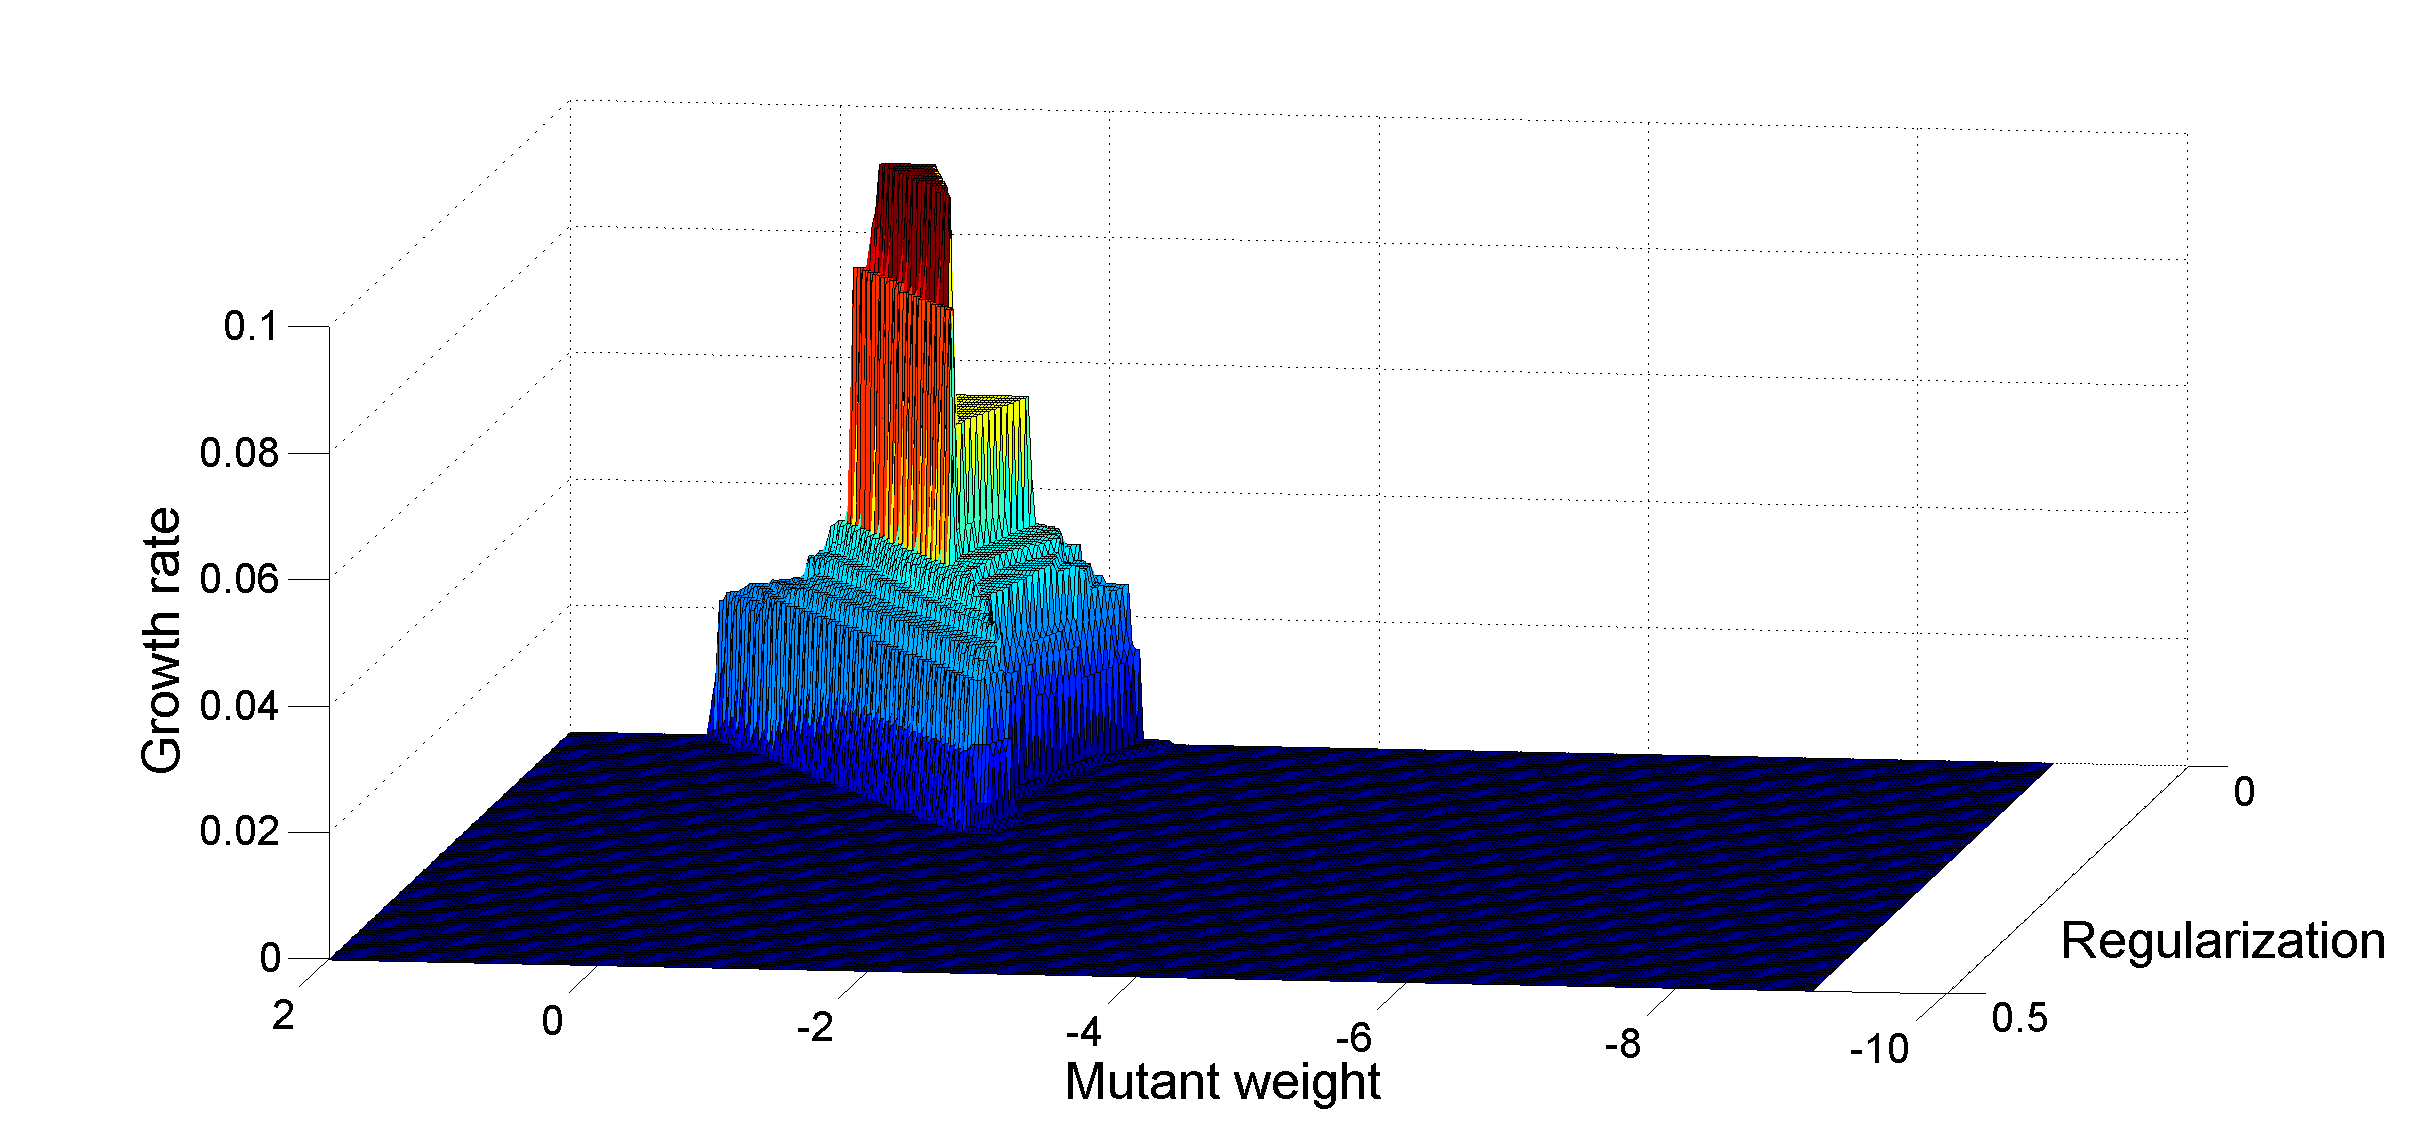
\includegraphics[width=\textwidth]{R264LP}
  \caption{Linear MoMA} 
  \label{fig:R264LP}
\end{subfigure}
\\
\begin{subfigure}[b]{\textwidth}
  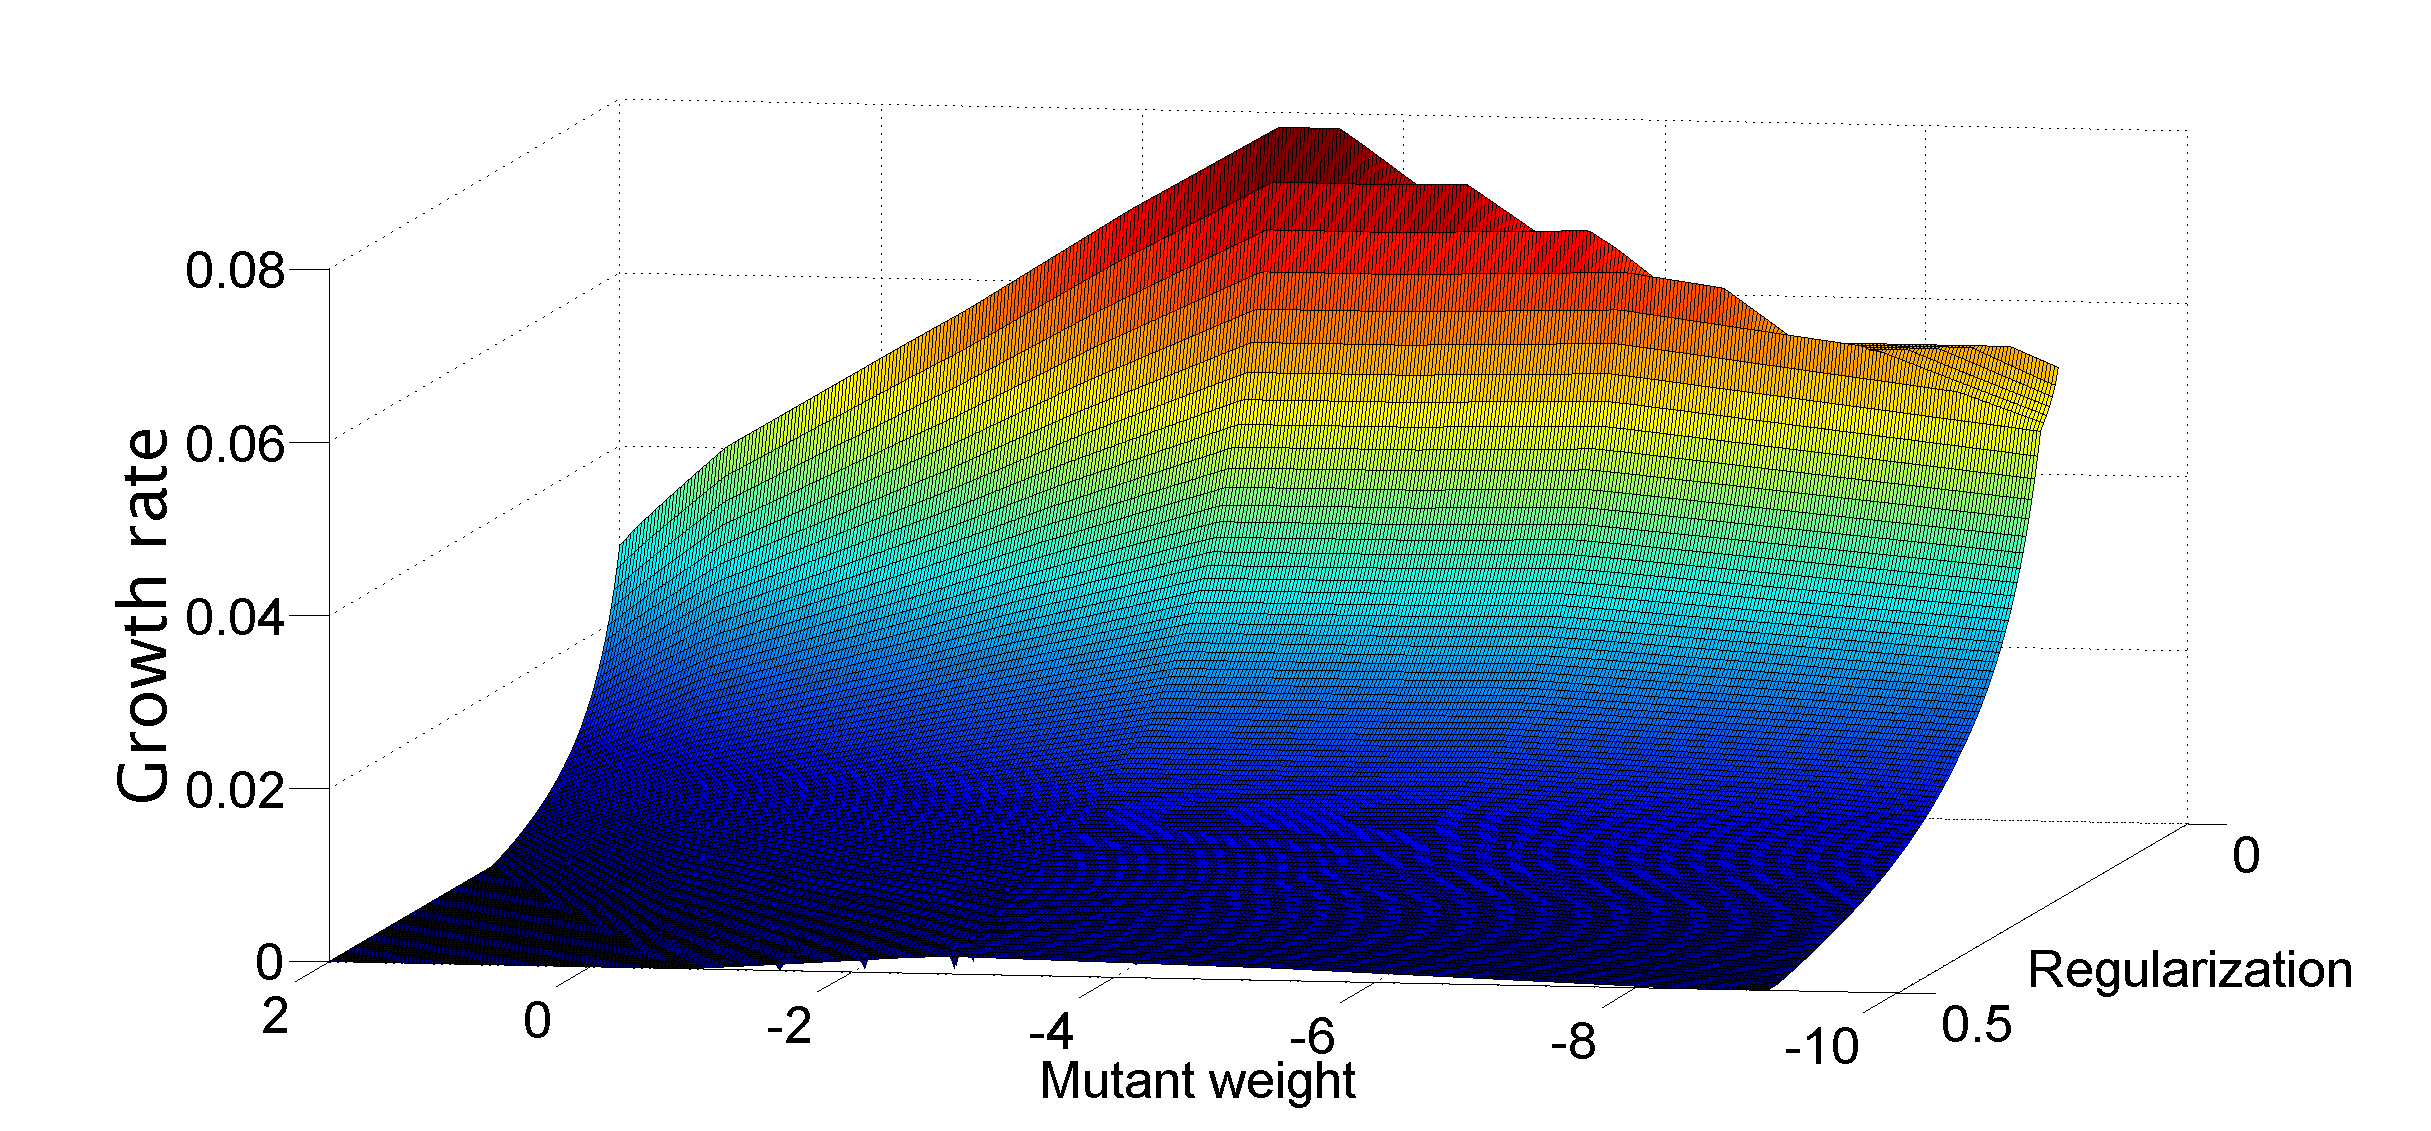
\includegraphics[width=\textwidth]{R264QP}
  \caption{Quadratic MoMA} 
  \label{fig:R264QP}
\end{subfigure}
\\
\end{tabular}
\caption{The same reaction is used in both figures, and in both
instances, a slightly negative weight on the reaction appears to be
most beneficial (compare to 0, which represents the wild-type).
Weight on a (linear or quadratic, respectively) 
regularization objective component is shown on the y-axis, which is often a helpful
constant both biologically and for removing invalid flux cycles 
\citep{Schuetz2012, Smallbone2009a}.}
\label{fig:wMoMA_smoothness}
\end{figure}

\section{Supporting Information}

\subsection{Evolutionary path analysis}
\label{sec:pathAnalysis}

The repository housing the project is currently located at:
\url{https://github.com/bbarker/COBRAscripts}. The C code which is
used for the analysis may be found in the
\texttt{MyProjects/AdaptiveMuts/TreeTraversal} subdirectory. 


The function we used to generate the combinatorial
mutation data is \texttt{randomEpistasisSampler} found in 
\texttt{MyProjects/AdaptiveMuts}. This function relies on another
function in the same directory for generating a pool of single
mutants, \texttt{randomSingleBeneMuts}.


